\documentclass[twoside]{../zirkelblatt1415}
\usepackage{mathtools}
\usepackage{wrapfig}
\usepackage{float}
\usepackage{booktabs}
\floatstyle{ruled}
\restylefloat{figure}
\restylefloat{table}
\let\raggedsection\centering
\newcommand{\RR}{\mathbb{R}}
\newcommand{\ZZ}{\mathbb{Z}}

\theoremstyle{definition}
\newtheorem{defn}{Definition}[section]
\newtheorem{defn'}{Vorläufge Definition}[section]
\newtheorem{axiom}[defn]{Axiom}
\newtheorem{bsp}[defn]{Beispiel}

\theoremstyle{plain}

\newtheorem{prop}[defn]{Proposition}
\newtheorem{motto}[defn]{Motto}
\newtheorem{wunder}[defn]{Wunder}
\newtheorem{ueberlegung}[defn]{Überlegung}
\newtheorem{lemma}[defn]{Lemma}
\newtheorem{kor}[defn]{Korollar}
\newtheorem{hilfsaussage}[defn]{Hilfsaussage}
\newtheorem{satz}[defn]{Satz}
\newtheorem{thm}[defn]{Theorem}

\theoremstyle{remark}
\newtheorem{bem}[defn]{Bemerkung}
\newtheorem{warnung}[defn]{Warnung}
\newtheorem{aufg}[defn]{Aufgabe}

\definecolor{darkred}{rgb}{0.7,0,0}
\definecolor{shadecolor}{rgb}{.95,.95,.95}

\newenvironment{listing}{
  \renewcommand*\theenumi{\arabic{enumi}}
  \renewcommand{\labelenumi}{\theenumi.}
  \begin{enumerate}\itemsep0em}{\end{enumerate}}

\newcommand{\BB}{\mathrm{BB}}
\newcommand{\defeq}{\vcentcolon=}
\newcommand{\ol}[1]{\overline{#1}}

%\newcommand{\loesung}[1]{\rotatebox{180}{\vbox{#1}}}
\newcommand{\loesung}[1]{#1}

\begin{document}

\maketitleCustom{Klassen 10/11/12}{\textbf{\textsf{%
  Analytische Zahlentheorie \\
  \normalsize Zirkelzettel vom 5. Dezember 2014}}}

{\renewcommand{\addvspace}[1]{\vskip0.6em}
\tableofcontents%
}

\section{Der Fundamentalsatz der Arithmetik}

\begin{defn}Eine \emph{Primzahl} ist eine positive natürliche Zahl, die
\emph{genau zwei} verschiedene positive Teiler besitzt.\end{defn}

Gemäß dieser Definition beginnt die Folge der Primzahlen also mit
\[ 2, \quad 3, \quad 5, \quad 7, \quad 11, \quad 13, \quad 17, \quad \ldots \]
Die Zahl~$1$ zählt nicht als Primzahl -- sie besitzt als einzigen Teiler sich
selbst und hat daher nicht zwei verschiedene Teiler.

\begin{thm}[Fundamentalsatz der Arithmetik]Jede positive natürliche Zahl lässt
sich auf eindeutige Art und Weise als Produkt von Primzahlen
schreiben.\end{thm}

\begin{proof}Sei eine beliebige natürliche Zahl~$n$ gegeben. Falls~$n$ eine
Primzahl ist, haben wir damit die gesuchte Zerlegung in Primfaktoren schon
gefunden. Falls~$n$ keine Primzahl ist, spaltet sich~$n$ in ein Produkt auf: $n
= a \cdot b$, und wir können mit der Suche nach einer Zerlegung bei~$a$ und~$b$
fortfahren.

Die Eindeutigkeitsaussage ist interessanter (Aufgabe~\ref{aufg:eindt}).\end{proof}

\begin{aufgabeShaded}{Primfaktorzerlegung der Eins}
Der Fundamentalsatz der Arithmetik behauptet, dass sich \emph{jede} positive
natürliche Zahl in Primfaktoren zerlegen lässt. Die Zahl~$1$ ist auch eine
solche positive natürliche Zahl. Siehst du, wie sich diese zerlegen lässt?

\emph{Hinweis:} Das ist etwas versteckt. Beachte, dass~$1$ keine Primzahl ist.
\end{aufgabeShaded}

\begin{aufgabeShaded}{Soll Eins eine Primzahl sein?}
Es gibt ein gutes mathematisches Argument, wieso es sinnvoll ist, die Eins
nicht als Primzahl zu definieren. Finde es!

\emph{Tipp:} Denke an die Eindeutigkeit der Primfaktorzerlegung. Was wäre, wenn
man die Zahl Eins als Primzahl zulassen würde?
\end{aufgabeShaded}

\begin{aufgabeShaded}{Eindeutigkeit der Primfaktorzerlegung}\label{aufg:eindt}
Mit dieser Aufgabe beweisen wir, dass die Zerlegung einer Zahl in Primfaktoren
bis auf Umordnung der Faktoren eindeutig ist. In Formeln ausgedrückt: Gilt
\[ p_1 \cdots p_n = q_1 \cdots q_m, \]
wobei~$p_1,\ldots,p_n$ und~$q_1,\ldots,q_m$ Primzahlen sind, so folgt schon~$n
= m$ (links und rechts stehen also gleich viele Faktoren) und jeder Faktor der
linken Seite tritt auch genau einmal auf der rechten Seite auf und umgekehrt.

\begin{enumerate}
\item Zeige zuerst: Teilt eine Primzahl~$p$ ein Produkt~$a \cdot b$, so
teilt~$p$ schon~$a$ oder~$p$ teilt~$b$. In Formeln:
\[ \text{Wenn $p \mid ab$, dann $p \mid a$ oder $p \mid b$.} \]

\emph{Tipp:} Das ist gar nicht so leicht. Verwende, dass die Zahlen~$a$ und~$p$
irgendeinen größten gemeinsamen Teiler~$d$ haben, und dass sich dieser in der
Form~$d = fa + gp$ für gewisse Zahlen~$f$ und~$g$ schreiben lässt. (Eine solche
Darstellung des größten gemeinsamen Teilers heißt \emph{Bézoutdarstellung}.
Dass es eine solche immer gibt, folgt aus dem \emph{euklidischen Algorithmus}.)

\item Beweise mit dem Resultat aus Teilaufgabe~a) die Eindeutigkeitsbehauptung.
\end{enumerate}
\end{aufgabeShaded}


\section{Irrationalität}

\begin{defn}Eine reelle Zahl~$x$ heißt genau dann \emph{rational}, wenn sie
sich als Quotient zweier ganzer Zahlen schreiben lässt: $x = a/b$ für gewisse
ganze Zahlen~$a$ und~$b$.\end{defn}

Dass nicht alle Zahlen rational sind, war eine erstaunliche Entdeckung im
fünften Jahrhundert~v.~Chr. Manche sehen diese Erkenntnis sogar als
Geburtsstunde der modernen Mathematik an.\footnote{Als Entdecker der
Irrationalität gilt der griechische Mathematiker Hippasos von Metapont. Er
erkannte, dass der \emph{goldene Schnitt} irrational ist. Damit erschütterte er
die Schule der Pythagoreer, denn diese waren von dem Kredo \emph{Alles ist
Zahl} überzeugt, wobei sie mit "`Zahl"' \emph{rationale Zahl} meinten.
Ironischerweise kam der goldene Schnitt auch noch im Erkennungszeichen der
Pythagoreer vor, dem Pentagramm.}

\begin{thm}Die Zahl~$\sqrt{2}$ ist nicht rational.\end{thm}

\begin{aufgabeShaded}{Irrationalität von Quadratwurzeln}
\begin{enumerate}
\item Beweise, dass~$\sqrt{2}$ nicht rational ist.

\emph{Tipp:} Gehe nach folgendem Muster vor. Angenommen,~$\sqrt{2}$ ist doch
rational. Nach Definition gibt es dann ganze Zahlen~$a$ und~$b$ mit~$\sqrt{2} =
a/b$. Quadrieren und Umstellen zeigt~$2 b^2 = a^2$. Überlege nun, wie oft der
Primfaktor~$2$ auf den beiden Seiten dieser Gleichung vorkommt.

\item Beweise, dass für jede Primzahl~$p$ die Zahl~$\sqrt{p}$ nicht rational
ist.

\item Beweise, dass für jede Zahl~$n$, in deren Primfaktorzerlegung mindestens
eine Primzahl ungerade oft vorkommt, die Zahl~$\sqrt{n}$ nicht rational ist.
\end{enumerate}
\end{aufgabeShaded}

\begin{aufgabeShaded}{Anschauliche Bedeutung von Quadratwurzeln}
Wenn Quadratwurzeln sehr seltsame Zahlen ohne praktische Bedeutung wären,
hätten die alten Griechen vielleicht die Entdeckung der Irrationalität nicht
ganz so schlimm gefunden. Tatsächlich aber kommen Quadratwurzeln in der
Geometrie überall vor: Finde eine geometrische Figur, deren Kantenlängen alle
ganze Zahlen sind, sodass eine weitere eingezeichnete Hilfslinie aber
irrationale Länge hat.
\end{aufgabeShaded}


\section{Die Unendlichkeit der Primzahlen}


\section{Die riemannsche~$\zeta$-Funktion}

\begin{center}
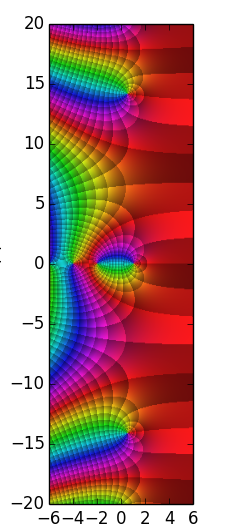
\includegraphics[angle=90]{zeta-function}
\end{center}


\end{document}
